%!TEX root = ../thesis.tex
\markboth{Appendix}{APPENDIX}
\begin{appendices}

\renewcommand\thefigure{A.\arabic{figure}}
\renewcommand\thetable{A.\arabic{table}}
\setcounter{figure}{0}
\setcounter{table}{0}

\subsection{DemoCut: Formative Study Material}

\begin{table}[h!]
   \begin{minipage}[b]{1.0\textwidth}
  \small
\begin{tabular}{| l | l | l | l | l | l |}
    \hline
    & & length & views & creation date & link\\ \hline
Electronics & 1 & 1:54:00 & 3006  & Oct 21, 2012  & \url{https://youtu.be/watch?v=zOBy6iKjpso} \\
  & 2 & 5:32:00 & 22211 & Sep 16, 2012  & \url{https://youtu.be/watch?v=4cuneFm-AG4} \\
  & 3 & 6:00:00 & 71895 & Jun 18, 2012  & \url{https://youtu.be/watch?v=hOdu1Zl1lic} \\
  & 4 & 5:34:00 & 130001  & Jun 30, 2011  & \url{https://youtu.be/watch?v=zYjOqcbBEco} \\ \hline
Home/Repair & 5 & 5:59:00 & 2231  & Oct 6, 2012 & \url{https://youtu.be/watch?v=Y5j55Mlg09s} \\
  & 6 & 8:40:00 & 5063  & Jan 4, 2013 & \url{https://youtu.be/watch?v=54k_OgAT_uQ} \\
  & 7 & 3:42:00 & 8312  & Mar 15, 2011  & \url{https://youtu.be/watch?v=JL5Q2lJAAdk} \\
  & 8 & 7:28:00 & 32201 & Mar 10, 2012  & \url{https://youtu.be/watch?v=7OrXrmFqXv0} \\ \hline
Art & 9 & 5:50:00 & 699177  & April 12, 2012  & \url{https://youtu.be/watch?v=RFauBl0zTvw} \\
  & 10  & 4:53:00 & 4004613 & Nov 18, 2011  & \url{https://youtu.be/watch?v=iybQwiJWToM} \\
  & 11  & 9:08:00 & 58248 & Aug 27, 2012  & \url{https://youtu.be/watch?v=va0sOYEHRho} \\
  & 12  & 2:26:00 & 6203  & Feb 8, 2013 & \url{https://youtu.be/watch?v=NHfPywNg_Vw} \\ \hline
Craft & 13  & 6:25:00 & 128741  & Jan 12, 2013  & \url{https://youtu.be/watch?v=RajOsFVWJ4I} \\
  & 14  & 3:09:00 & 19303 & Jan 22, 2013  & \url{https://youtu.be/watch?v=8KP-trX9I5g} \\
  & 15  & 4:17:00 & 1156  & Oct 5, 2012 & \url{https://youtu.be/watch?v=ajW6h6JAR04} \\
  & 16  & 2:32:00 & 2804  & Feb 2, 2013 & \url{https://youtu.be/watch?v=qBUJtRNUGOA} \\ \hline
Food  & 17  & 2:16:00 & 130752  & Jun 4, 2009 & \url{https://youtu.be/watch?v=3opfBL9YZ10} \\
  & 18  & 8:14:00 & 30740 & Apr 11, 2011  & \url{https://youtu.be/watch?v=DWxUa9LwbSY} \\
  & 19  & 3:47:00 & 22670 & Sep 12, 2011  & \url{https://youtu.be/watch?v=l0QHDHMe9oU} \\
  & 20  & 3:54:00 & 9192  & Feb 6, 2012 & \url{https://youtu.be/watch?v=5G3OGIN7Cx8} \\ \hline
\end{tabular}
\end{minipage}

\vspace{10pt}
Available at \url{https://www.youtube.com/playlist?list=PLAq2QZEiIgn80wbHOp9In4s8IzDnkb3II}

\caption{20 YouTube How-To videos used in the formative user study.}
  \label{tab:democut_formative}
\end{table}

\clearpage

\subsection{DemoDraw: User Study Material and Results}

\begin{figure}[h!]
     \centering
    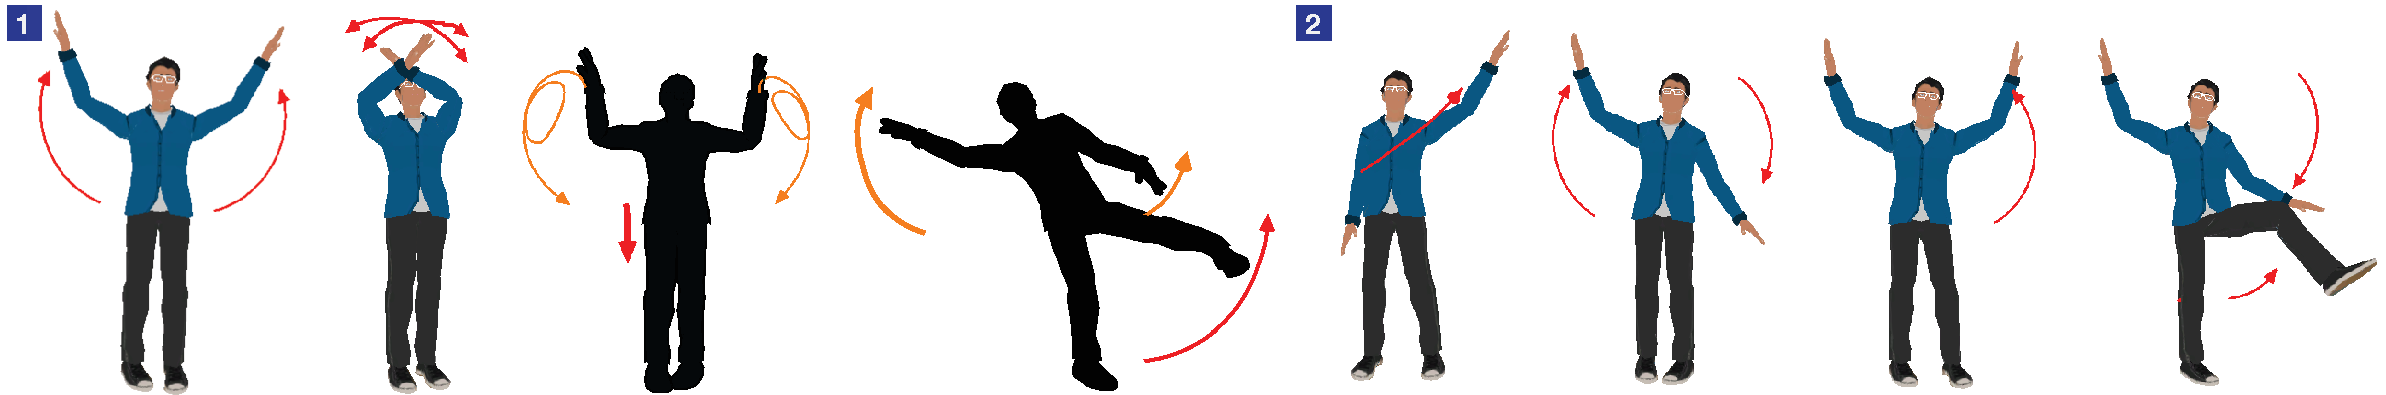
\includegraphics[width=\columnwidth]{\demodraw/fig/study1/study1_tasks}
    \caption{Tasks provided in Study 1: We showed the printouts of these two sets of 4-step motions generated by DemoDraw using both the Demonstration Interface and the Refinement Interface. We asked participants to re-perform in front of a camera.}
    \label{fig:study_review_tasks}
 \end{figure}

   \vspace{6mm}
\begin{figure}[h!]
     \centering
    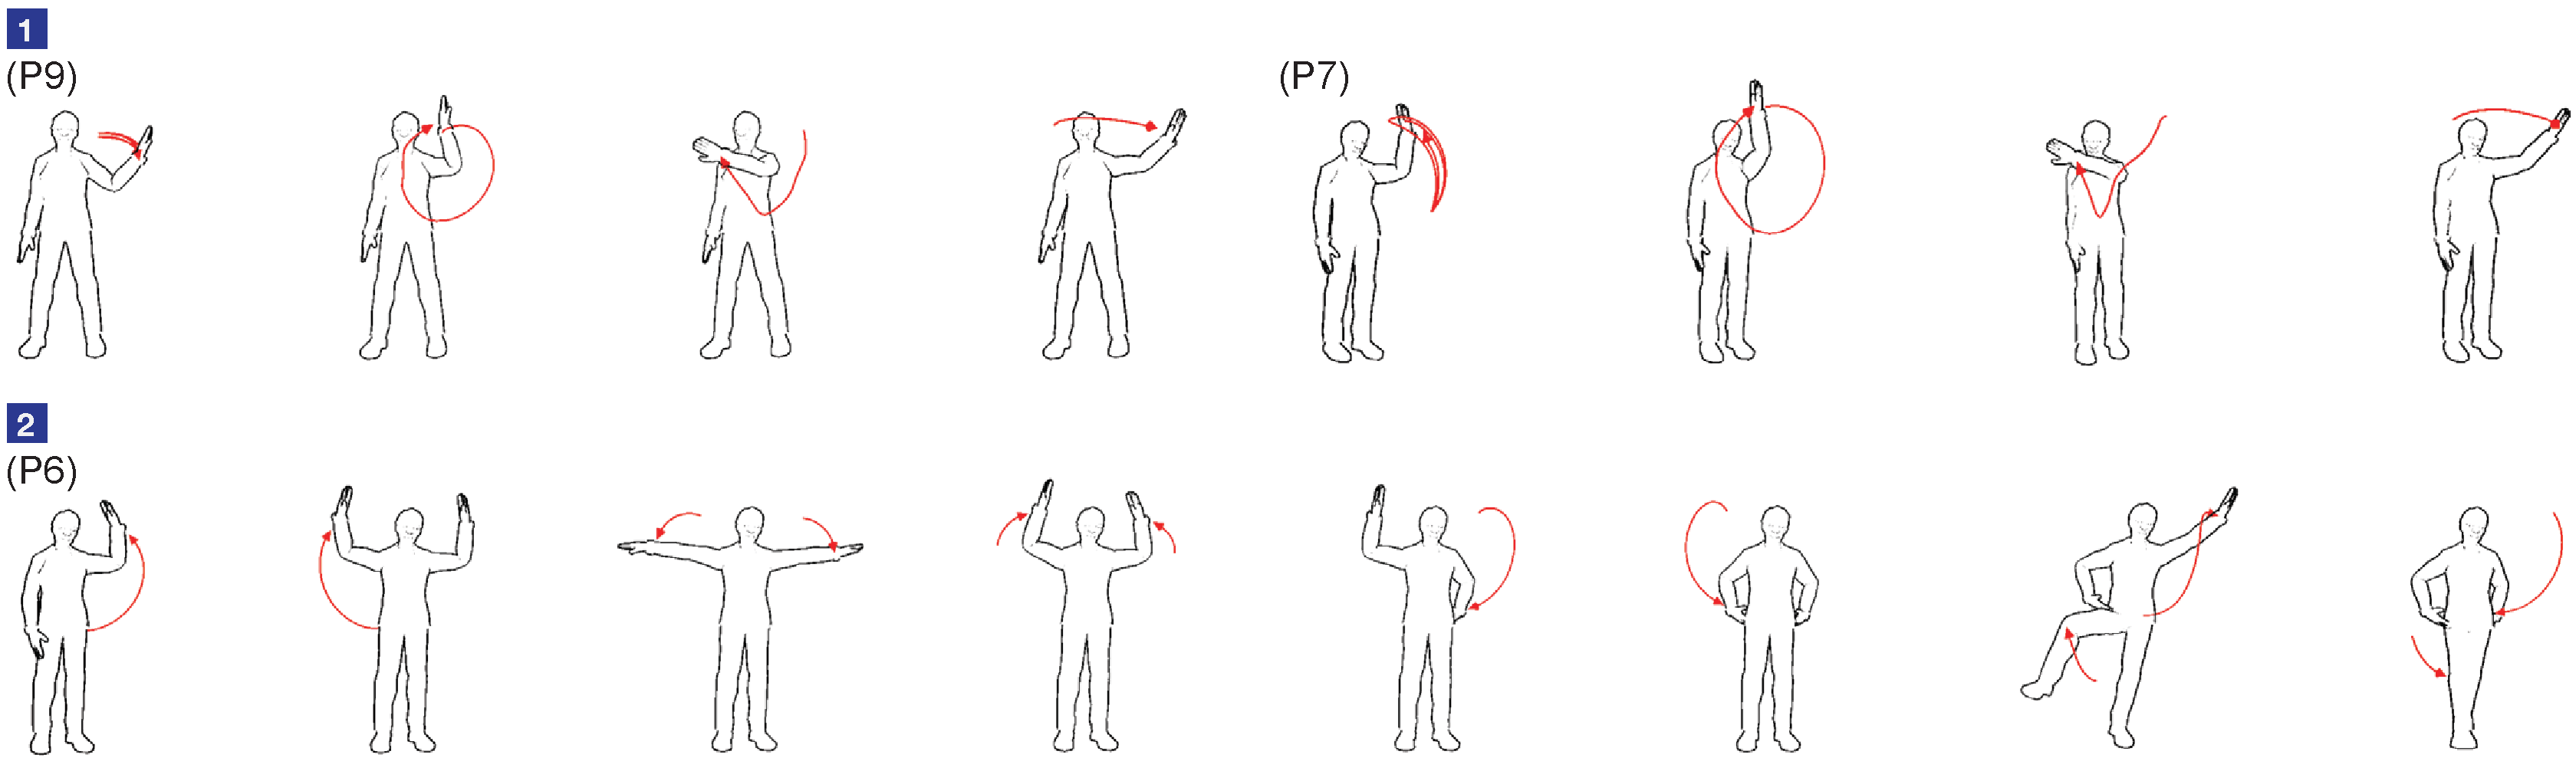
\includegraphics[width=\columnwidth]{\demodraw/fig/study2/study2_tasks}
    \caption{Step-by-step illustrations generated by participants in Study 2 using the \phaseI{}: 1) Results from P9 and P6 showing the same four gestures of a gestural interface in task 1, and 2) Results from P6 showing 8-step moves in task 2.}
    \label{fig:study_authoring_tasks}
   \end{figure}

   \vspace{6mm}
\begin{figure}[h!]
     \centering
    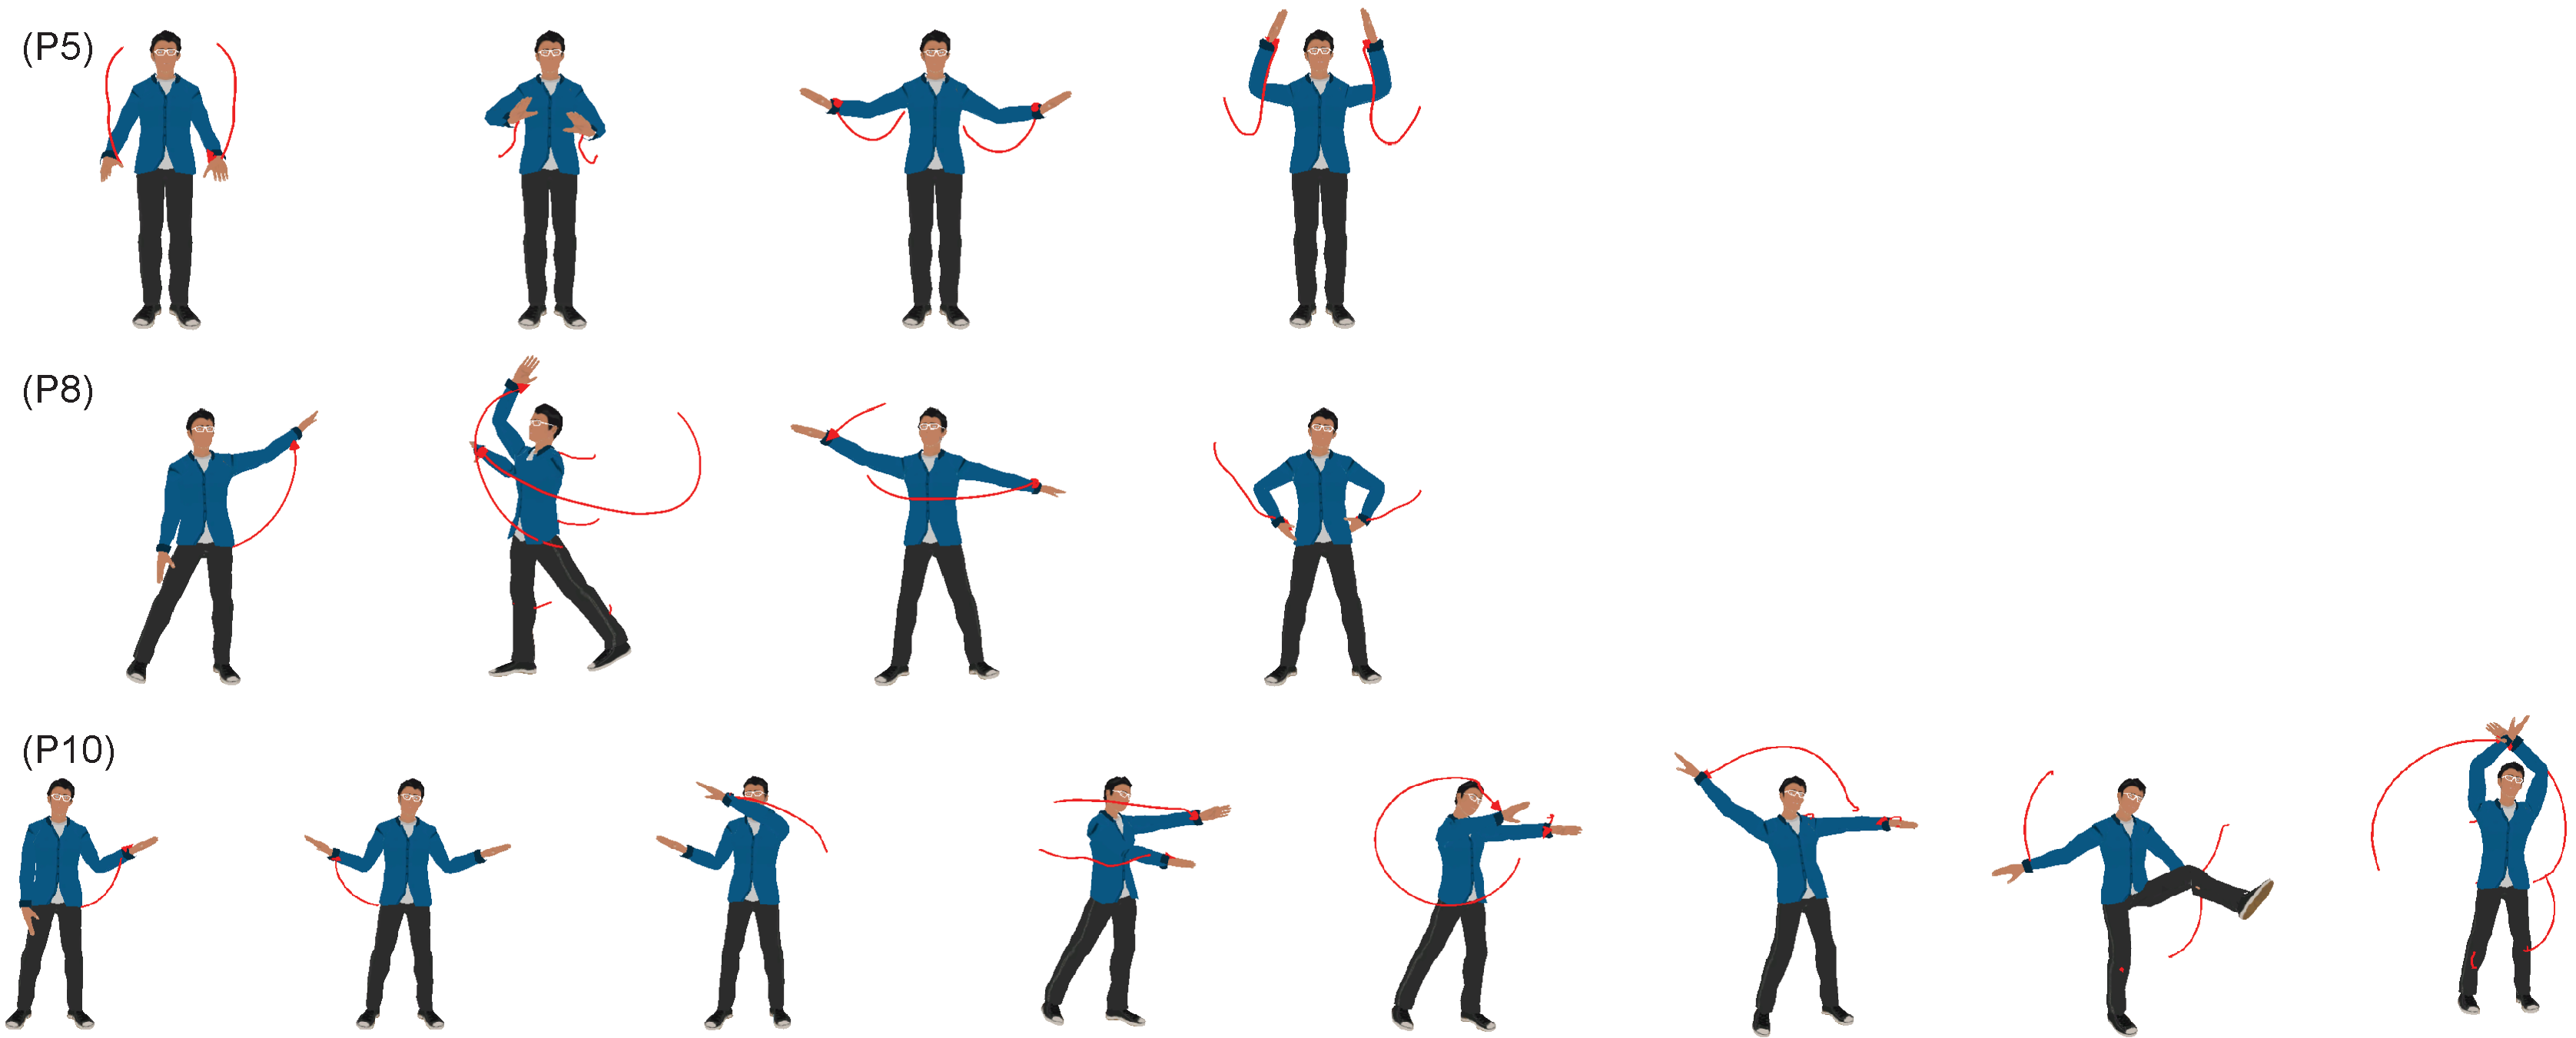
\includegraphics[width=\columnwidth]{\demodraw/fig/study2/study2_open}
    \caption{Selected illustrations from the open-ended task created by three different participants using the using Demonstration Interface in Study 2: P5 performed to conduct a 4/4 beat pattern; P8 and P10 each performed four and eight free moves.}
    \label{fig:open_ended_examples}
 \end{figure}

\end{appendices}
